% Wiring diagram of the Bop-It game. Build: pdflatex fig-wiring.tex, then copy the PDF to ../fig-wiring.pdf
\documentclass[border=4pt]{standalone}
\usepackage[T1]{fontenc}
\usepackage{mathptmx}
\usepackage{tikz}
\begin{document}
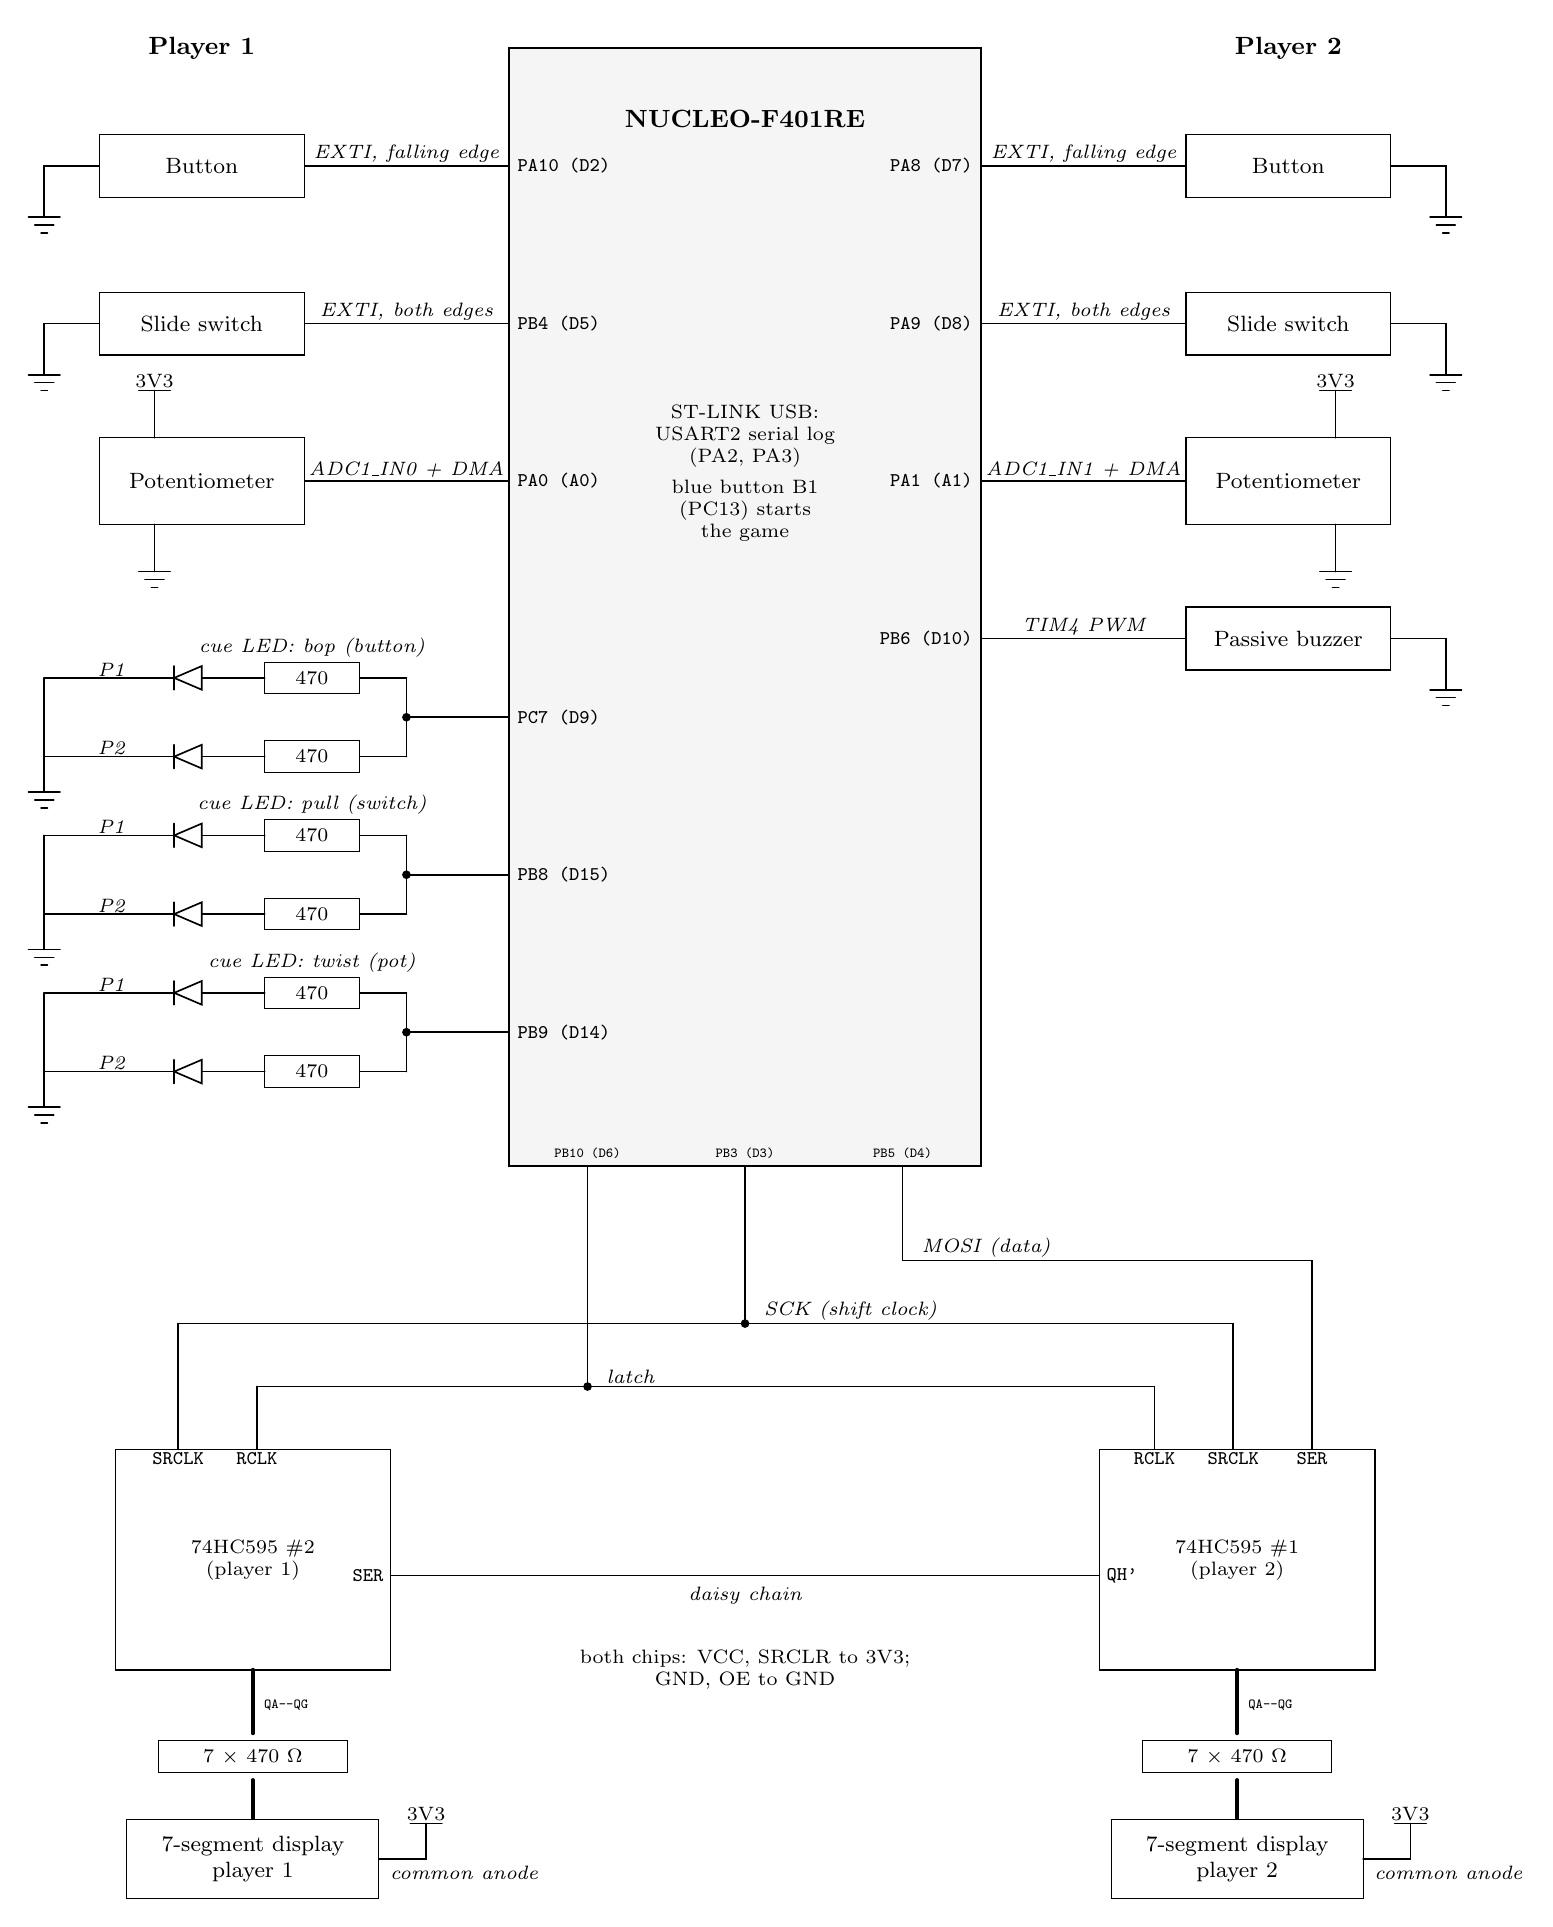
\begin{tikzpicture}[font=\footnotesize, line cap=round,
  wire/.style={line width=0.6pt},
  bus/.style={line width=1.6pt},
  comp/.style={draw, fill=white, minimum width=2.6cm, minimum height=0.8cm, align=center, inner sep=2pt},
  res/.style={draw, fill=white, minimum width=1.2cm, minimum height=0.4cm, inner sep=1pt, font=\scriptsize},
  wl/.style={font=\scriptsize\itshape, inner sep=1pt},
  pn/.style={font=\scriptsize\ttfamily, inner sep=1pt},
  head/.style={font=\small\bfseries}]

% ---------- symbols ----------
\newcommand{\gnd}[2]{\draw[wire] (#1,#2)--(#1,#2-0.15);
  \draw[wire] (#1-0.2,#2-0.15)--(#1+0.2,#2-0.15);
  \draw[wire] (#1-0.12,#2-0.25)--(#1+0.12,#2-0.25);
  \draw[wire] (#1-0.04,#2-0.35)--(#1+0.04,#2-0.35);}
\newcommand{\vcc}[2]{\draw[wire] (#1,#2)--(#1,#2+0.15); \draw[wire] (#1-0.2,#2+0.15)--(#1+0.2,#2+0.15);
  \node[font=\scriptsize, anchor=south, inner sep=1pt] at (#1,#2+0.15) {3V3};}
\newcommand{\jdot}[2]{\fill (#1,#2) circle (0.055);}

% button, switch, buzzer: pin -- component -- GND   (side = -1 left, +1 right)
\newcommand{\simplerow}[4]{%
  \pgfmathsetmacro{\xa}{#1*3.0}\pgfmathsetmacro{\xb}{#1*5.6}\pgfmathsetmacro{\xc}{#1*6.9}
  \pgfmathsetmacro{\xd}{#1*8.2}\pgfmathsetmacro{\xe}{#1*8.9}\pgfmathsetmacro{\xm}{#1*4.3}
  \draw[wire] (\xa,#2)--(\xb,#2);
  \node[comp] at (\xc,#2) {#3};
  \draw[wire] (\xd,#2)--(\xe,#2)--(\xe,#2-0.5);
  \gnd{\xe}{#2-0.5}
  \node[wl, anchor=south] at (\xm,#2) {#4};}

% potentiometer: 3V3 -- pot -- GND, wiper to the pin
\newcommand{\potrow}[4]{%
  \pgfmathsetmacro{\xa}{#1*3.0}\pgfmathsetmacro{\xb}{#1*5.6}\pgfmathsetmacro{\xc}{#1*6.9}
  \pgfmathsetmacro{\xt}{#1*7.5}\pgfmathsetmacro{\xm}{#1*4.3}
  \draw[wire] (\xa,#2)--(\xb,#2);
  \node[comp, minimum height=1.1cm] at (\xc,#2) {#3};
  \draw[wire] (\xt,#2+0.55)--(\xt,#2+1.0); \vcc{\xt}{#2+1.0}
  \draw[wire] (\xt,#2-0.55)--(\xt,#2-1.0); \gnd{\xt}{#2-1.0}
  \node[wl, anchor=south] at (\xm,#2) {#4};}

% shared cue LED: two LEDs (player 1 and 2) in parallel, 470 ohm each
\newcommand{\ledrow}[2]{%
  \draw[wire] (-3.0,#1)--(-4.3,#1);
  \draw[wire] (-4.3,#1+0.5)--(-4.3,#1-0.5);
  \jdot{-4.3}{#1}
  \foreach \dy/\who in {0.5/P1,-0.5/P2}{
    \pgfmathsetmacro{\yy}{#1+\dy}
    \draw[wire] (-4.3,\yy)--(-4.9,\yy);
    \node[res] at (-5.5,\yy) {470};
    \draw[wire] (-6.1,\yy)--(-6.9,\yy);
    \draw[wire, fill=white] (-6.9,\yy+0.15)--(-6.9,\yy-0.15)--(-7.25,\yy)--cycle;
    \draw[wire] (-7.25,\yy+0.15)--(-7.25,\yy-0.15);
    \draw[wire] (-7.25,\yy)--(-8.9,\yy);
    \node[wl, anchor=south] at (-8.05,\yy-0.02) {\who};
  }
  \draw[wire] (-8.9,#1+0.5)--(-8.9,#1-0.8); \gnd{-8.9}{#1-0.8}
  \node[wl, anchor=south] at (-5.5,#1+0.72) {#2};}

% ---------- Nucleo ----------
\draw[thick, fill=gray!8] (-3,-6.2) rectangle (3,8);
\node[font=\small\bfseries, align=center] at (0,7.1) {NUCLEO-F401RE};
\node[font=\scriptsize, align=center] at (0,2.6) {ST-LINK USB:\\USART2 serial log\\(PA2, PA3)\\[3pt]blue button B1\\(PC13) starts\\the game};

\foreach \y/\n in {6.5/PA10 (D2), 4.5/PB4 (D5), 2.5/PA0 (A0), -0.5/PC7 (D9), -2.5/PB8 (D15), -4.5/PB9 (D14)}
  \node[pn, anchor=west] at (-2.93,\y) {\n};
\foreach \y/\n in {6.5/PA8 (D7), 4.5/PA9 (D8), 2.5/PA1 (A1), 0.5/PB6 (D10)}
  \node[pn, anchor=east] at (2.93,\y) {\n};
\foreach \x/\n in {-2/PB10 (D6), 0/PB3 (D3), 2/PB5 (D4)}
  \node[pn, anchor=south, font=\tiny\ttfamily] at (\x,-6.15) {\n};

% ---------- player 1 (left) ----------
\node[head] at (-6.9,8) {Player 1};
\simplerow{-1}{6.5}{Button}{EXTI, falling edge}
\simplerow{-1}{4.5}{Slide switch}{EXTI, both edges}
\potrow{-1}{2.5}{Potentiometer}{ADC1\_IN0 + DMA}

% ---------- cue LEDs (left, shared by both players) ----------
\ledrow{-0.5}{cue LED: bop (button)}
\ledrow{-2.5}{cue LED: pull (switch)}
\ledrow{-4.5}{cue LED: twist (pot)}

% ---------- player 2 (right) ----------
\node[head] at (6.9,8) {Player 2};
\simplerow{1}{6.5}{Button}{EXTI, falling edge}
\simplerow{1}{4.5}{Slide switch}{EXTI, both edges}
\potrow{1}{2.5}{Potentiometer}{ADC1\_IN1 + DMA}
\simplerow{1}{0.5}{Passive buzzer}{TIM4 PWM}

% ---------- 74HC595 chain ----------
% buses: data (y=-7.4), clock (y=-8.2), latch (y=-9.0)
\draw[wire] (2,-6.2)--(2,-7.4)--(7.2,-7.4)--(7.2,-9.8);
\draw[wire] (0,-6.2)--(0,-8.2); \jdot{0}{-8.2}
\draw[wire] (-7.2,-8.2)--(6.2,-8.2)--(6.2,-9.8);
\draw[wire] (-7.2,-8.2)--(-7.2,-9.8);
\draw[wire] (-2,-6.2)--(-2,-9.0); \jdot{-2}{-9.0}
\draw[wire] (-6.2,-9.0)--(5.2,-9.0)--(5.2,-9.8);
\draw[wire] (-6.2,-9.0)--(-6.2,-9.8);
\node[wl, anchor=south west] at (2.2,-7.4) {MOSI (data)};
\node[wl, anchor=south west] at (0.2,-8.2) {SCK (shift clock)};
\node[wl, anchor=south west] at (-1.8,-9.0) {latch};

% chip 1 (right, player 2), chip 2 (left, player 1)
\draw[fill=white] (4.5,-12.6) rectangle (8,-9.8);
\node[font=\scriptsize, align=center] at (6.25,-11.2) {74HC595 \#1\\(player 2)};
\node[pn, anchor=north] at (5.2,-9.8) {RCLK}; \node[pn, anchor=north] at (6.2,-9.8) {SRCLK}; \node[pn, anchor=north] at (7.2,-9.8) {SER};
\draw[fill=white] (-8,-12.6) rectangle (-4.5,-9.8);
\node[font=\scriptsize, align=center] at (-6.25,-11.2) {74HC595 \#2\\(player 1)};
\node[pn, anchor=north] at (-7.2,-9.8) {SRCLK}; \node[pn, anchor=north] at (-6.2,-9.8) {RCLK};
% daisy chain: QH' of chip 1 -> SER of chip 2
\draw[wire] (4.5,-11.4)--(-4.5,-11.4);
\node[pn, anchor=west] at (4.55,-11.4) {QH'}; \node[pn, anchor=east] at (-4.55,-11.4) {SER};
\node[wl, align=center, anchor=north] at (0,-11.5) {daisy chain};
\node[font=\scriptsize, align=center] at (0,-12.6) {both chips: VCC, SRCLR to 3V3;\\GND, OE to GND};

% segment lines and displays
\foreach \cx/\who in {6.25/2, -6.25/1}{
  \draw[bus] (\cx,-12.6)--(\cx,-13.4);
  \node[res, minimum width=2.4cm] at (\cx,-13.7) {7 $\times$ 470 $\Omega$};
  \draw[bus] (\cx,-14.0)--(\cx,-14.5);
  \node[pn, anchor=west, font=\tiny\ttfamily] at (\cx+0.1,-13.05) {QA--QG};
  \node[comp, minimum width=3.2cm, minimum height=1cm] (d\who) at (\cx,-15.0) {7-segment display\\player \who};
  \draw[wire] (\cx+1.6,-15.0)--(\cx+2.2,-15.0)--(\cx+2.2,-14.7); \vcc{\cx+2.2}{-14.7}
  \node[wl, anchor=north west] at (\cx+1.7,-15.05) {common anode};
}
\end{tikzpicture}
\end{document}
